\documentclass[a4paper,12pt]{article}
\usepackage[OT1]{fontenc}
\usepackage{graphicx,pifont}
\usepackage{epsfig,amsmath,amssymb,url}
\usepackage{multicol}
\usepackage[english]{babel}
\usepackage{csquotes}
\usepackage{hyperref}
\usepackage{lipsum}
\usepackage{graphicx}
\usepackage{bibentry}
\usepackage[maxbibnames=99,maxcitenames=2,style=apa,giveninits=true,uniquename=false,apamaxprtauth=999]{biblatex}
\addbibresource{references.bib}
\usepackage[document]{ragged2e}
\usepackage{blindtext}
\setlength{\parindent}{0pt}
\setlength{\parskip}{2ex plus 0.5ex minus 0.2ex}
\linespread{1.2}
\tolerance2000
\hoffset=-0.5cm
\setlength{\textwidth}{15.5cm}
%\voffset=0cm
\setlength{\textheight}{620pt}



\begin{document}

\pagestyle{empty}

\begin{center}
REPORT IN SRILANKAN ECONOMIC CRISIS \\

\vspace*{.5cm}

{\Large SRILANKAN ECONOMIC CRISIS
\\
}

\vspace*{2cm}

{\large
AHMED REZA RIDAY    \hspace{3.4cm}  ID:200101022\\
MD. SHOWMIK HASAN    \hspace{3.1cm}    ID:200101034\\
HUZAIFA HASSAN    \hspace{4.3cm}     ID:200101003\\
SHAFEIN SADIA ISLAM    \hspace{3cm}   ID:200101045\\
BONNHI SIKHA DUTTA    \hspace{3cm}   ID:200101029\\
MD. MOSTOFA WADUD    \hspace{3cm}   ID:200101020\\
}
\vspace*{1cm}
\graphicspath{ {./images/} }

\includegraphics{baust 1}

%Institute for Atmospheric and Earth System Research / Physics\\
Department of Computer Science And Engineering \\
Faculty of Electrical And Computer Engineering \\
Bangladesh Army University Of Science And Technology \\
Saidpur, Bangladesh

\vspace*{.5cm}

{\em To be presented for public discussion with the permission of the Faculty of Electrical And Computer Engineering
}

\vspace*{1cm}

{\bf Bangladesh 2022}

\newpage
\vspace*{-2.2cm}

\begin{tabular}{ll}
Author's Address:
& Bangladesh Army University Of Science And Technology \\
& P.O. Box 5310 \\
& ahmedrezashams4@gmail.com \\
\\
Supervisors:
& Lecturer Md. Al Hasan, Ph.D.\\
& Department Of Computer Science And Engineering\\%
& Bangladesh Army University Of Science And Technology\\
\\
%& Professor Firstname Lastname, Ph.D.\\
%& Institute for Atmospheric and Earth System Research / Physics\\
%& University of Helsinki\\
\\
Reviewers:
& Professor Hasan Mohammad Kafi, Ph.D.\\
& Department of Computer Science And Engineering\\
& Bangladesh Army University Of Science And Technology \\
\
%& Associate Professor Firstname Lastname, Ph.D.\\
%& Laboratory of XX\\
%& University of XX\\
\\
%Opponent:
%& Professor Firstname Lastname, Ph.D. \\
%& Institute of XX \\
%& University of XX
\end{tabular}

\vfill

%\begin{multicols}{2}
%ISBN  xxx-xxx-xxxx-xx-x (printed) \\
%ISSN xxxx-xxxx \\
%Helsinki YYYY \\
%Unigrafia Oy

%ISBN  xxx-xxx-xxxx-xx-x (pdf) \\
%ISSN xxxx-xxxx \\
%Helsinki YYYY \\
%http://www.FAAR.fi
%\end{multicols}
\end{center}
\newpage

\large
\justifying
The thesis titled \textbf{"Srilankan Economic Crisis"} submitted by Ahmed Reza Riday (200101022) has  been accepeted as satisfactory in partial fulfillment of the requirement for the degree of B.Sc. Engineering in Computer Science And Engineering(CSE) to be awarded by the Bangladesh Army University Of Science and Technology (BAUST) on 15-May,2022.

\newpage
\centering\section*{Board Of Examiners}
\begin{tabular}{ll}
\large
1.\\
Head of the Department\\
Designation : Associate Professor\\
Department Of Computer Science And Engineering(CSE)\\
Bangladesh Army University Of Science And Technology(BAUST)\\
\\
2.\\
Name of the Supervisor\\
Designation :Assistant Professor \\
Department Of Computer Science And Engineering(CSE)\\
Bangladesh Army University Of Science And Technology(BAUST)\\
\\
3.\\
Name of the Member\\
Designation :Assistant Professor \\
Department Of Computer Science And Engineering(CSE)\\
Bangladesh Army University Of Science And Technology(BAUST)\\
\\
\end{tabular}
\vfill
\newpage
\centering\section*{CANDIDATE DECLARATION}
\justifying
It is hereby declared that this thesis or any part of it has not been submitted elsewhere for the award of any degree or deploma.\\
\vspace{2cm}\newline
\textbf{
\- - - - - - - - - - - - - - - - - - - - \\
1.Signature of the Candidate \newline 
Date: \newline
\vspace{1cm}\newline
\- - - - - - - - - - - - - - - - - - - - \\
2.Signature of the Candidate \newline
Date: \newline \\
\vspace{1cm}\newline
\- - - - - - - - - - - - - - - - - - - - \\
3.Signature of the Candidate \newline
Date: \newline \\
\vspace{1cm}\newline
\- - - - - - - - - - - - - - - - - - - - \\
4.Signature of the Candidate \newline
Date: \newline \\
\vspace{1cm}\newline
\- - - - - - - - - - - - - - - - - - - - \\
5.Signature of the Candidate \newline
Date: \newline \\
\vspace{1cm}\newline
\- - - - - - - - - - - - - - - - - - - - \\
6.Signature of the Candidate \newline
Date: \newline \\
}
\newpage
\section{Acknowledgement}
\vspace*{-0.7cm}
\justifying
\large
First and foremost, we would like to thank Almighty Allah for enabling us to initiate the research, to put our best efforts and successfully conclude it. Secondly, we submit our heartiest gratitude to our respected Supervisor Md. Al-Hasan, Lecturer, Department of Computer Science and Engineering in Bangladesh Army University of Science and Technology for his contribution, guidance and support in conducting the research and preparation of the report. Starting from instilling in us the deadliest of fears to the kindest words of inspiration has permitted us to effectively complete the paper. We are truly grateful to him. We revere the patronage and moral support extended with love, by our parents as well as our friends. They helped us with their direct or indirect suggestions which aided in achieving our goal. We would also like to acknowledge the assistance we received from numerous resources over the Internet especially from fellow researchers’ work.
The thesis has also benefited from the comments and suggestions made by Prof. Hasan Muhammad Kafi ,Assistant Professor , Computer Science and Engineering, Bangladesh Army University of Science and Technology. We want to take this opportunity to thanks him.

For extended discussion and valuable suggestions which have contributed greatly to the improvement of the thesis and to read through the manuscript we would like to thank 
Dr. Mohammed Sowket Ali, Assistant Professor, Computer Science and Engineering, Bangladesh Army University of Science and Technology.

Last but not the least, we would like to thank our beloved "Bangladesh Army University of Science and Technology" for providing a nice environment of study and research with its enriched faculty members which helped us greatly in completing our bachelor degree. 




\newpage
\vspace*{-1cm}\section*{Abstract}
\justifying
The Sri Lankan economic crisis is an ongoing crisis in the island nation of Sri Lanka that started in 2019 to become the nation's worst economic situation since its independence in 1948.It has led to unprecedented levels of inflation, near-depletion of foreign exchange reserves, shortages of medical supplies and an increase in prices of basic commodities.The crisis has said to have been caused by multiple compounding factors including tax cuts, money creation, a nationwide policy to shift to organic or biological farming and events such as the Easter bombings in 2019 and the impact of the COVID-19 pandemic. The subsequent economic hardships resulted in the public openly voicing their dissent, leading to the 2022 Sri Lankan protests.

Sri Lanka had been earmarked for sovereign default, as the remaining foreign reserves of USD 1.9 billion as of March 2022 would not be sufficient to pay the country's foreign debt obligations for 2022, with USD 4 billion to be repaid.An International Sovereign Bond repayment of USD 1 billion is also due to be paid by the government in July 2022. Bloomberg reported that Sri Lanka had a total of USD 8.6 billion in repayments due in 2022, including both local debt and foreign debt.In April 2022, the Sri Lankan government announced that it was defaulting, making it the first sovereign default in Sri Lankan history since its independence in 1948.

Keywords: Foreign exchange reserves, Economic crisis, Impact of the COVID-19 pandemic, Sovereign default, Hot money.\newline

\newpage

\setlength{\parskip}{0.5ex plus 0.5ex minus 0.2ex}

\small\tableofcontents
\setlength{\parskip}{2ex plus 0.5ex minus 0.2ex}
\newpage

%%\section*{List of publications}

%This thesis consists of an introductory review, followed by XX
%research articles.  In the introductory part, these papers are cited
%according to their roman numerals.

%%\begin{description}
%%\item[\bf I.]{\fullcite{paperOne2020}}
%%\item[\bf II.]{\fullcite{paperTwo2021}}
%%\item[\bf III.]{\fullcite{paperThree2022}}
%%\item[\bf IV.]{\fullcite{paperFour2022}}
%%\end{description}

%Add here a statement about article reprinting rights.

\newpage

\pagestyle{plain}

\section{Introduction}\label{introduction}
\subsection{OVERVIEW}
\large
Sri Lanka had been earmarked for sovereign default, as the remaining foreign exchange reserves of USD 1.9 billion as of March 2022 would not be sufficient to pay the country's foreign debt obligations for 2022, with USD 4 billion to be repaid.An International Sovereign Bond repayment of USD 1 billion is also due to be paid by the government in July 2022. Bloomberg reported that Sri Lanka had a total of USD 8.6 billion in repayments due in 2022, including both local debt and foreign debt.In April 2022, the Sri Lankan government announced that it was defaulting, making it the first sovereign default in Sri Lankan history since its independence in 1948.\newline
The Sri Lankan economic crisis is an ongoing crisis in the island nation of Sri Lanka that started in 2019 to become the nation's worst economic situation since its independence in 1It has led to unprecedented levels of inflation, near-depletion of foreign exchange reserves, shortages of medical supplies and an increase in prices of basic commodities.The crisis has said to have been caused by multiple compounding factors including tax cuts, money creation, a nationwide policy to shift to organic or biological farming and events such as the Easter bombings in 2019 and the impact of the COVID-19 pandemic. The subsequent economic hardships resulted in the public openly voicing their dissent, leading to the 2022 Sri Lankan protests.
%\subsection{MOTIVATION}
\subsection{BACKGROUND}
According to W. A. Wijewardena, a former Deputy Governor of the Central Bank of Sri Lanka, the country was a long way into an economic crisis in 2015. The government which came into power in 2015 knew this and had been warned by the Institute of Policy Studies of Sri Lanka of a number of risks. While then Prime Minister Ranil Wickremesinghe in 2015 had presented a strong economic policy to address the situation, the coalition government could not get the policy pushed through Parliament which would eventually result in further policy confusion in the coming months. The government did not adequately address the economic warnings and emerging dangers, consuming itself in other government related activities such as "constitutional reforms". Certain practices, including those by the Ministry of Finance led by Ravi Karunanayake, were globally frowned upon. Election related economic decisions were pushed such as excessive distribution of freebies. The Institute of Policy Studies of Sri Lanka's 2014 State of the Economy Report highlighted hot money, worrying borrowing practices, temporary and superficial quick-fixes and monopoly of FDI flow into one sector, viz. hospitality. Further political turmoil in 2018 worsened the economic outlook. By that time, the government had carried out several reforms under an IMF supported program towards fiscal monetary consolidation and had successfully controlled inflation. These reforms included an automatic fuel pricing formula which significantly reduced fiscal risks posed by state-owned enterprises (SOEs), raised the for Value Added Tax (VAT) rate from 11 percent to 15 percent and broadened the VAT base by removing exemptions. Many of the reforms were reversed by the new government after the 2019 elections.\newline
\centering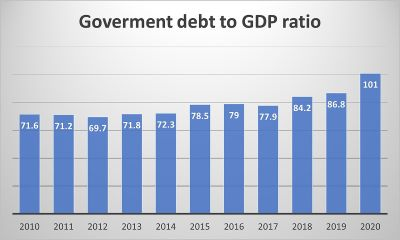
\includegraphics[]{images/Government_debt_to_GDP_ratio.jpg}
\justifying
The last administration also drafted the 2019 Central Bank Bill to make the Central Bank independent from political influence by banning the Treasury Secretary and any member of the Government from becoming members of the Monetary Board. Money printing was also to be banned as the bill states “The Central Bank shall not purchase securities issued by the government, by any government-owned entity, or any other public entity in the primary market,”. Then Central Bank Governor, Dr. Indrajit Coomaraswamy noted Balance of Payments issues, increased inflation and asset bubbles as reasons for the ban. The Sri Lanka Podujana Party led by the Rajapaksas opposed an independent Central Bank and discarded the bill as soon as they came to power.

Many experts compared Lebanon's economic situation with that of Sri Lanka and had warned that Sri Lanka too was on the way to defaulting on its sovereign bonds. Both nations had similar issues, including deep economic crises occurring after their successive governments piled up unsustainable debts following the end of civil wars.
%\subsection{LITERATURE REVIEW}
\subsection{SUMMARY}
Debt in billions due to years of accumulated borrowings, record inflation, lack of foreign currency, crucial sectors witnessing a sharp fall in demand thanks to the pandemic, and the alleged government mismanagement are among the reasons that have dragged Sri Lanka into not just an unprecedented economic crisis but also a massive political turmoil.
%\href{https://www.overleaf.com/learn/latex/Bibliography_management_with_biblatex}{\texttt{biblatex}} package. Examples of in-text citations: \cite{paperOne2020} found something \parencite[e.g.][]{paperTwo2021}.

\section{Causes}

\subsection{Tax cuts and money creation}
The Government of Sri Lanka under president Gotabaya Rajapaksa made large tax cuts that affected government revenue and fiscal policies, causing budget deficits to soar. These cuts included increased tax-free thresholds that resulting in a 33.5\% decline in registered taxpayers, reducing VAT to 8\%, reducing corporate tax from 28\% to 24\%, the abolishment of the Pay As You Earn (PAYE) tax and the 2\% “nation-building tax” which financed infrastructure development. The massive loss of tax revenue resulted in rating agencies downgrading the sovereign credit rating making it harder to take more debt. In 2021 P. B. Jayasundera stated that President Rajapaksa was aware of the loss of revenue but considered it an "investment" and have no plans to increase taxes for another 5 years.To cover government spending, the Central Bank began printing money in record amounts, ignoring advice from the International Monetary Fund (IMF) to stop printing money and instead hike interest rates and raise taxes while cutting spending. The IMF warned that continuing to print money would lead to an economic implosion. The tax cuts were also opposed by the former Finance Minister Mangala Samaraweera who noted that as the Sri Lankan government already had far less tax revenue relative to most countries which combined with its high debt load tax cuts would be dangerous. Samaraweera predicted that “If these proposals are implemented like this not only will the entire country go bankrupt, but the entire country will become another Venezuela or another Greece.”

On 6 April 2022, the CBSL allegedly printed 119.08 billion rupees, making it the highest reported amount printed on a single day by the CBSL for the year 2022. The total money added to financial markets for the year 2022 increased to Rs. 432.76 billion.

\subsection{External debt}
Since 2010, Sri Lanka's foreign debt more than doubled between 2010 and 2020. While foreign debt was about 42\% of the GDP in 2019, it rose to 119\% of its GDP in 2021.[failed verification][dubious – discuss] By the end of 2022, the country is due to pay USD 4 billion to debtors, whereas in April 2022, government reserves amounted for USD 2.3 billion.

Despite commentaries blaming China for the debt crisis, the Australian Lowy Institute pointed out that Sri Lanka was "not engulfed in a Chinese debt trap", because external debt owed to China was only about 10\% of the debt stock in April 2021. Instead, the majority of Sri Lanka's external debt stock is owed to international capital markets, which accounted for 47\%. Another 22\% is held by multilateral development banks, followed by Japan having 10\% of Sri Lankan external debt. In January 2022, President Gotabhaya Rajapaksa's office stated that it would appeal to China to reschedule its debt burden during talks with the Chinese foreign minister Wang Yi. As of March 2022, there has been no official response from China.\newline

In 2020, S\&P Global Ratings said Sri Lanka's existing funding sources did not appear sufficient to cover its debt servicing needs, estimated at just over 4.0\$ billion in 2021. According to the agency Bellwether, "To solve Sri Lanka's 'budgetary problem' in repaying debt, Treasuries auctions have to succeed. When that is done, the 'transfer problem' of foreign exchange will be automatically solved... Instead, with failed Treasury bill auctions filled with printed money, the country is slipping deeper into debt." To resolve the debt crisis, Bellwether noted that Sri Lanka would need a credible fiscal plan and monetary policy, increasing taxes to repay debt, and interest rates and opening of imports would allow taxes to flow back to the Treasury. While it is possible to raise rates and generate dollars to repay the foreign debt by curtailing domestic credit, it is not practical to do it on an ongoing basis for many years. If investors see foreign reserves going up after debt repayments, confidence may come back but it is a painful affair, which may or may not work given the current ideology.

In September 2021, the government announced an economic emergency, as the situation was further aggravated by the falling national currency exchange rate, inflation rising as result of high food prices, and pandemic restrictions in tourism which further decreased the country's income.[35] This drove Sri Lanka to the brink of bankruptcy due to foreign reserves falling to US 1.9\$ billion as of March 2022, this being insufficient to pay the foreign debt obligations of US 4\$ billion and an International Sovereign Bond (ISB) payment of US 1\$ billion for the year 2022. The national inflation rate increased to 17.5\% in February 2022, according to the National Consumer Price Index.

The government repaid US 500\$ million International Sovereign Bonds which was due in January 2022 despite growing opposition came from economic analysts and experts who all advised the government to postpone the ISB payment in order to preserve the foreign reserves.

On 12 April 2022, Sri Lanka announced that it will be defaulting on its external debt of 51\$ billion.

\subsection{Fall of foreign remittances}
The Central Bank of Sri Lanka under Cabraal attempted to maintain the LKR pegged while continuing heavy money printing and strict exchange controls thus pushing down the market value of rupee. Thus, by February 2022 while the government attempted to keep the currency pegged at 200 LKR to the USD unofficial market value of the LKR was exceeding 248 to the US dollar. Thus, foreign workers went on remitting money through unofficial channels causing Sri Lankan banks to run out of foreign currency and foreign remittances to crash with a 61\% reduction in official remittances in January 2022. In turn Cabraal threatened to freeze bank accounts of those that use unofficial money transmission methods. Then Cabraal began targeting merchandise and services exporters with exporter dollar surrender requirements forcing the residual after the utilization of export proceeds to be converted into LKR and forcefully converting dollars in forex accounts of resident Sri Lankans who earn dollar salaries ignoring concerns of this creating a similar situation to remittances. As Banks struggled, Cabraal issued warning letters to CEOs of banks demanding strict adherence to the fixed conversion rate. Former Deputy Governor of CBSL W.A Wijeywardana criticized the policies calling it "Cabraalnomics 2.0" noting that the dollars are disappearing from official markets while a superior dynamic black market has caused exporters and immigrants to shun the formal banking system resulting in dismantling the power of the Central Bank as the forex regulator.

\subsection{Agricultural crisis}
The Central Bank of Sri Lanka under Cabraal attempted to maintain the LKR pegged while continuing heavy money printing and strict exchange controls thus pushing down the market value of rupee. Thus, by February 2022 while the government attempted to keep the currency pegged at 200 LKR to the USD unofficial market value of the LKR was exceeding 248 to the US dollar. Thus, foreign workers went on remitting money through unofficial channels causing Sri Lankan banks to run out of foreign currency and foreign remittances to crash with a 61\% reduction in official remittances in January 2022. In turn Cabraal threatened to freeze bank accounts of those that use unofficial money transmission methods. Then Cabraal began targeting merchandise and services exporters with exporter dollar surrender requirements forcing the residual after the utilization of export proceeds to be converted into LKR and forcefully converting dollars in forex accounts of resident Sri Lankans who earn dollar salaries ignoring concerns of this creating a similar situation to remittances. As Banks struggled, Cabraal issued warning letters to CEOs of banks demanding strict adherence to the fixed conversion rate. Former Deputy Governor of CBSL W.A Wijeywardana criticized the policies calling it "Cabraalnomics 2.0" noting that the dollars are disappearing from official markets while a superior dynamic black market has caused exporters and immigrants to shun the formal banking system resulting in dismantling the power of the Central Bank as the forex regulator.
\subsection{Russo-Ukrainian War}
The repercussions of the ongoing tense situation between Ukraine and Russia due to the Russo-Ukrainian War is felt in the already sluggish economic conditions of Sri Lanka. The 2022 Russian invasion of Ukraine has further exacerbated the economic calamity of the country as Russia is the second biggest market to Sri Lanka in tea exports and Sri Lanka's tourism sector is heavily reliant upon these two nations as most of the tourist arrivals are from Russia and Ukraine. As a result, the Ukrainian crisis has put a halt to the path of economic recovery of Sri Lanka with both tea and tourism sector have been hit hard.
\section{Impact}

\subsection{Electricity and fuel shortages}
The economic crises has resulted in declines in electricity, fuel and cooking gas consumption, resulting from shortages. Finance Minister Basil Rajapaksa urged all government authorities to switch off all street lights at least up until the end of March 2022 in an attempt to conserve electricity. Nearly 1000 bakeries have been shut as a response to shortages of cooking gas. Long queues have formed in recent months in front of petrol filling stations. The surge in global oil prices further aggravated the fuel shortage. In order to conserve energy, daily power cuts have been imposed by the authorities throughout the country. On 22 March 2022, the government ordered the military to post soldiers at various gas and fuel filling stations to curb the tensions among people who line up in queues and to ease the fuel distribution. Casualties include four fatalities due to fatigue and violence. Daily seven hour power cuts were seen throughout March 2022, increased to 10 hours at the end of the month and again Increased to 15 hours in Early April. The dailies The Island and Divaina stopped print publication due to paper shortages and related price escalation and switched to e-papers. Sri Lanka's hydroelectricity generation has also been affected.

\subsection{Education Sector}
In March 2022, several schools in Sri Lanka announced that their term/mid-year examinations would be postponed indefinitely, due to paper shortages throughout the country mainly triggered due to the lack of foreign reserves to import paper. The term test examinations were stated to be held island-wide on 28 March 2022, but due to the acute shortage of printing paper and ink ribbons, a decision was made to either cancel or postpone the exams to a later date.
\subsection{Health}
On 29 March, all scheduled surgeries at the Peradeniya Teaching Hospital were suspended due to a shortage of medicines.

Many other hospitals have also apparently suspended routine surgeries and have also reduced a large number of laboratory tests. Other state-run hospitals were also reported to be running out of life-saving medicines. On 8 April, the Medical Council of Sri Lanka issued a warning that there would be a catastrophic number of deaths, which is likely to be in excess of the combined death toll of COVID-19, the 2004 tsunami and the Civil War, unless a replenishment of supplies is made in a matter of weeks. Singapore Red Cross Society issued warning declaring Sri Lanka's medical crisis as an "unprecedented humanitarian crisis".

By 10 April, hospitals had begun to run out of endotracheal tubes for the ventilation of new-born babies, infants and children. Doctors requested that overseas Sri Lankan communities provide neonatal ETTs of sizes 4mm, 3.5mm, 3mm, 2.5mm, and 2mm. The Sri Lanka Medical Association said that all hospitals in the country no longer had access to imported medical tools and vital drugs. Hospitals were pushed to the extent that they decided to sterilize and reuse endotracheal tubes to deliver oxygen to the lungs of newborn babies.

Doctors are reported to have been forced to reuse old and used medical equipment to treat the patients due to the shortage of new equipment. Doctors are also reported to have performed medical surgeries by using the light of mobile phones. Doctors in rural areas have also been forced to stitch wounds in the dark due to rolling power cuts. The emergency drugs to treat heart attacks are also reported to be in short supply.
\subsection{Tourism}
The country's tourism sector represented over one-tenth of the GDP of Sri Lanka. The sector was negatively affected by the 2019 Easter bombings, and the COVID-19 pandemic prevented recovery. According to the World Bank in April 2021, "Despite the heavy toll of the COVID-19 pandemic on Sri Lanka's economy and the lives of its people, the economy will recover in 2021, though challenges remain."

In March 2022, the United Kingdom and Canada warned their travellers to be aware of the current economic situation in Sri Lanka.

\section{Government responses}
\subsection{Monetary Policy}
The Rajapaksa Government initially denied existence of any crisis and refused to seek assistance from the IMF. CBSL Governor Cabraal also criticized rating downgrades by Moody's as unwarranted, erroneous and reckless. By March 2022 the Government while accepted the existence of the economic crisis denied any responsibility and Gotabaya Rajapaksa in a speech blamed his critics for creating the crisis which was echoed by the Central Bank under Cabraal who blamed the media, the opposition's "doomsday reports", rating agencies and the COVID-19 pandemic for causing the crisis. In April 2022 President Rajapaksa accepted the agricultural crisis and the refusal to seek IMF assistance early on as "mistakes".

On 8 April 2022, the Central Bank of Sri Lanka further tightened the monetary policy (contractionary monetary policy) to curtain soaring inflation by raising both the Standing Lending Facility Rate and Standing Deposit Facility Rate by 700 basis points.
\subsection{Fiscal Policy}
On 30 April 2022 the Finance Minister Ali Sabry claimed that the government is looking to increase taxes accepting that the tax cuts in 2019 were a mistake. The 8\% VAT was termed "definitely not sustainable" for Sri Lanka and claimed that the rate should be around 13-14\%.
\section{Gradually Fall Of A Country}

\subsection{Foreign Loan}
Sri Lanka, the island nation in the Indian Ocean with a population of nearly 22 million, has plunged into a deep economic crisis. With more than 50\$ billion (€46 billion) in external debt and a shortage of foreign exchange reserves, the country is currently struggling to pay for essential imports. This has led to sharp increases in the price of essential commodities like rice, fuel, and milk. A fuel shortage recently left much of the country suffering through a 13-hour power cut.

Sri Lanka's foreign debt obligations for this year exceed 7\$ billion. But the country's forex reserves as of March 2022 is just 1.6\$ billion. On Tuesday, the country announced a default on all its foreign debt. Now Sri Lanka is hoping for an IMF bailout to save it from the worsening crisis. 
\subsection{Crashed GDP}
\begin{center}
\begin{tabular}{|c c  c|}

 \hline
 Year & GDP Nominal & GDP Change \\ [0.5ex] 
 \hline\hline
 2021 & \$84.5 billion & 4.1\% \\ 
 \hline
 2020 & \$80.71 billion & -3.6\% \\ 
 \hline
 2019 & \$83.98 billion & 2.3\% \\ 
 \hline
 2018 & \$87.95 billion  & 3.2\% \\ 
 \hline
 2017 & \$87,357,205,923 & 3.4\% \\
 \hline
 2016 & \$81,787,420,023 & 4,47\% \\
 \hline
 2015 & \$80,604,080,689 & 5.01\% \\
 \hline
 2014 & \$79,356,449,841 & 4.96\% \\ [1ex] 
 \hline
\end{tabular}
\end{center}
\centering{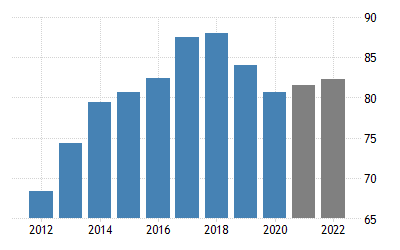
\includegraphics{images/sri-lanka-gdp.png}}\\
\newpage
\justifying
\subsection{Learning For Bangladesh}
In terms of economic indicators, Bangladesh is in a much more comfortable position than Sri Lanka. However, economic experts are asking whether the current state will persist for another four-five years.
Professor Muinul Islam, Ekushey Padak-winning economist and former teacher of Chittagong University, said Bangladesh is in no imminent danger but is concerned by the unnecessary projects the country has started.
%{\bf Paper I.} \lipsum[75]

%{\bf Paper II.} \lipsum[75]

%{\bf Paper III.} \lipsum[75]

%{\bf Paper IV.} \lipsum[75]

\section{Conclusions}
The Sri Lankan government sought aid from the US, India and China. India has extended a \$1 billion line of credit for the supply of essential commodities already. And financial assistance of \$2.4 billion has also been provided by our country since January. 

Let’s just hope that the “Go Gota Go” by Sri Lankan protesters comes to fruition. 
\newpage
\begin{thebibliography}{00}
\bibitem{b1} Wikipedia, the free encyclopedia, ``Economy of Sri Lanka'' 
\bibitem{b2} https://www.economist.com/asia/sri-lankas-economic-crisis-has-created-a-political-one/21808595.
\bibitem{b3} https://indianexpress.com/article/world/sri-lanka-economic-crisis-live-updates-protests-rajapaksa-7865253/.
\bibitem{b4} Shibly,FHA, `` Economic Crisis And Its Impact On Economic Development,'' unpublished.
\bibitem{b5}Prema-chandra Athukorala, Edimon Ginting,
Hal Hill, and Utsav Kumar, ``The Srilanakan Economy,'' J. Name Stand. Abbrev., in press.

\end{thebibliography}
\end{document}
